\documentclass[twocolumn]{svjour3}          % twocolumn

\usepackage{cite}
\usepackage{graphicx}
\usepackage{url}

% KR: remove before submitting
\usepackage{color}
\usepackage{soul}
\newcommand{\myedit}[2]{\textcolor{red}{\st{#1}} \textcolor{blue}{#2}}
\newcommand{\marginnote}[1]{\marginpar{\scriptsize\emph{\textbf{\textcolor{red}{#1}}}\normalsize}}

% Insert the name of "your journal" with
\journalname{Environmental Earth Sciences}
%
\begin{document}

\title{TESSIN VISLab - Laboratory for Scientific Visualization%\thanks{Grants or other notes
%about the article that should go on the front page should be
%placed here. General acknowledgments should be placed at the end of the article.}
}
%\subtitle{Do you have a subtitle?\\ If so, write it here}

%\titlerunning{Short form of title}        % if too long for running head



\author{Lars Bilke         \and
        Thomas Fischer     \and
        Carolin Helbig     \and
        Thomas Kalbacher   \and
        Olaf Kolditz       \and
        Dmitry Naumov      \and
        Karsten Rink       \and
        Agnes Sachse       \and
        Benny Selle        \and
        Alexander Singer   \and
        Feng Sun           \and
        Nico Trauth        \and
        Marc Walther       \and
        Norihiro Watanabe  \and
        Bj\"orn Zehner     \and
        Jennifer Ziesch
}

%\authorrunning{Short form of author list} % if too long for running head

\institute{L. Bilke \and T. Fischer \and C. Helbig \and T. Kalbacher \and O. Kolditz \and
           Dmitry Naumov \and Karsten Rink \and Agnes Sachse \and Alexander Singer
           \and Nico Trauth \and Marc Walther \and Norihiro Watanabe \at
              Department of Environmental Informatics, \\
              Helmholtz Centre for Environmental Research, \\
              Leipzig, Germany, \\
              \email{lars.bilke@ufz.de}           %  \\
%             \emph{Present address:} of F. Author  %  if needed
           \and
           O. Kolditz \at
              Applied Environmental System Analysis, \\
              Technische University at Dresden, \\
              Dresden, Germany
           \and
           B. Selle \at
           \and
           F. Sun \at
              Beijing Hydrological Center, \\
              Beijing, China
           \and
           B. Zehner \at
              Bundesanstalt für Geowissenschaften und Rohstoffe, \\
              Hannover, Germany
           \and
           J. Ziesch \at
              Leibniz Institute for Applied Geophysics, \\
              Hannover, Germany
}

\date{Received: date / Accepted: date}
% The correct dates will be entered by the editor


\maketitle

\begin{abstract}
Scientific visualization is an integral part of the modeling workflow, enabling researchers to understand complex or large datasets and simulation results. A high-resolution stereoscopic virtual reality (VR) environment further enhances the possibilities of visualization. Such an environment also allows to collaborate in work groups including people of different backgrounds and to present results of a research project to stakeholders or the public. The requirements for the computing equipment driving the VR environment require specialized software applications which can be run in a parallel fashion on a set of interconnected machines. Another challenge is to devise a useful data workflow from source datasets onto the display system. Therefore we develop software applications like the \emph{OpenGeoSys Data Explorer} and custom data conversion tools for established visualization packages such as \emph{\myedit{ParaView}{Unity}} and \emph{VTK}. We demonstrate our workflow by presenting visualization results for case studies from a broad range of applications. An outlook on how visualization techniques can be deeply integrated into the simulation process is given and future technical improvements such as a simplified hardware setup and useful interaction techniques are outlined.

\keywords{Virtual Reality  \and  Visualization  \and  Computer Graphics}
\end{abstract}

%%%%%%%%%%
%% CONTENT
%%%%%%%%%%

\section{Introduction}
\label{introduction}

\myedit{}{Hier m\"usste eigentlich noch Motivation hin, wie super wichtig wiss. Visualisierung ist (Wiederholung aus Abstract + ein bisschen mehr + Quellenangaben. Am besten inkl. ein paar VR Dinge.}

TODO: Die beiden folgenden Abschnitte zusammenfuehren:

Using numerical models for the assessment of current and future states of real world applications, aiding in the evaluation of various management options, has become a standard -- not only in environmental sciences. Proper tools are needed to visualize the data properly for analyzing and investigating measurements and modeling results. With nowadays increasing density of available data and concurrently more and more detailed model setups, this need has grown strongly.

Climate change is one of the world's biggest challenges for the future. To predict these changes, meteorologists proceed in developing models that simulate the state of the atmosphere for a period of time. With an increasing of computational power, even the complexity of these models and their spatial resolution rises and produces large datasets with numerous variables (e.g.~wind, mass fraction). Scientific visualization is an essential medium to explore, analyze and present these datasets.

\section{TESSIN VISLab}
\label{tessin-vislab}

\myedit{}{Der folgende Absatz + die Stichpunktliste k\"onnte evtl schon mit in die n\"achste Section. Nachdem du in der Motivation ein bisschen was zu VR allgemein schreibst, sagst du, dass total viele Leute das schon erkannt haben wie wichtig das ist und dass in x, y und z VR-Zentren aufgebaut wurden. Wir haben auch eins und dann der folgende Absatz und dann der Technical Overview.}
\bigskip

The \emph{TESSIN VISLab} is a high-resolution immersive virtual reality (VR) environment and was established in 2008 to face the need of analyzing and working on increasingly complex datasets generated by simulations of natural phenomena in environmental sciences. Typical use cases for this environment are:

\begin{itemize}
\itemsep1pt\parskip0pt\parsep0pt
\item
  collaborative discussions in small groups of scientists
\item
  exploring complex datasets
\item
  verifying the quality of datasets
\item
  showing concurrent visualizations of heterogeneous integrated datasets
\item
  presenting research results to stakeholders
\item
  presentations for the general public such as on open house events
\end{itemize}

\subsection{Existing vislabs}
\label{existing-vislabs}

\myedit{}{Definiere was ein VisLab eigentlich ist! (bzw. Was du hier drunter verstehst)}

\begin{itemize}
\itemsep1pt\parskip0pt\parsep0pt
\item
  Potsdam
\item
  Zuse Berlin
\item
  Magdeburg
\item
  Aachen
\end{itemize}

\subsection{Technical Overview}
\label{technical-overview}

The hardware setup of the \emph{TESSIN VISLab} (TODO figure) uses a back projection-based stereoscopic visualization environment with an approximately 6x3 meter large main screen and extending projections on the floor and two side wings. In order to achieve a high resolution of approximately 6400 by 1800 pixels, 13 projectors are used. Images are generated alternating for the left and the right eye and users wear special glasses which separate these images, resulting in a stereoscopic view. For the stereo separation we can switch between two technologies -- active stereo using shutter glasses~\cite{activestereo} and passive stereo using \emph{Infitec} technology~\cite{infitec}. We use an optical tracking system, compensating for movement of the observer. An optical motion tracking system~\cite{tracking} based on infrared cameras detecting passive markers on the user's 3D glasses allows to compute images such that a correct perspective is maintained. Additionally a pointer device (\emph{Flystick}) allows for interaction with the virtual environment. The rendering is performed using a cluster with 13 workstations (one for each projector) equipped with high-end NVidia graphics boards (GPUs) and situated in a server room next to the presentation venue. The master / server process of the actual application is started on a hardware device in front of the display that allows to control multiple machines in the server room from one keyboard, mouse and monitor (\emph{KVM switch}). In addition to the virtual reality capabilities, the \emph{VISLab} can be employed for enhanced multimedia presentations such as the simultaneous display of images, videos and documents or a combination of 2D and 3D content. A typical use case is to present the 3D data on the main screen and additional datasets such as images, spreadsheets, maps and videos in a context-dependent way on the two side screens~\cite{zehner:modelcare}.

\subsection{Mobile VR equipment}
\label{mobile-vr-equipment}

For off-site presentations such as on conferences, workshops or visits to project partners or stakeholders, we can also utilize mobile equipment to demonstrate the same visualization projects as in the \emph{VISLab}. The equipment consists of notebooks with dedicated GPUs and 3D-enabled projectors or head-mounted displays (\emph{HMDs}) such as the \emph{Oculus Rift}~\cite{web:rift} (see figure \ref{fig:rift}).

\begin{figure}
  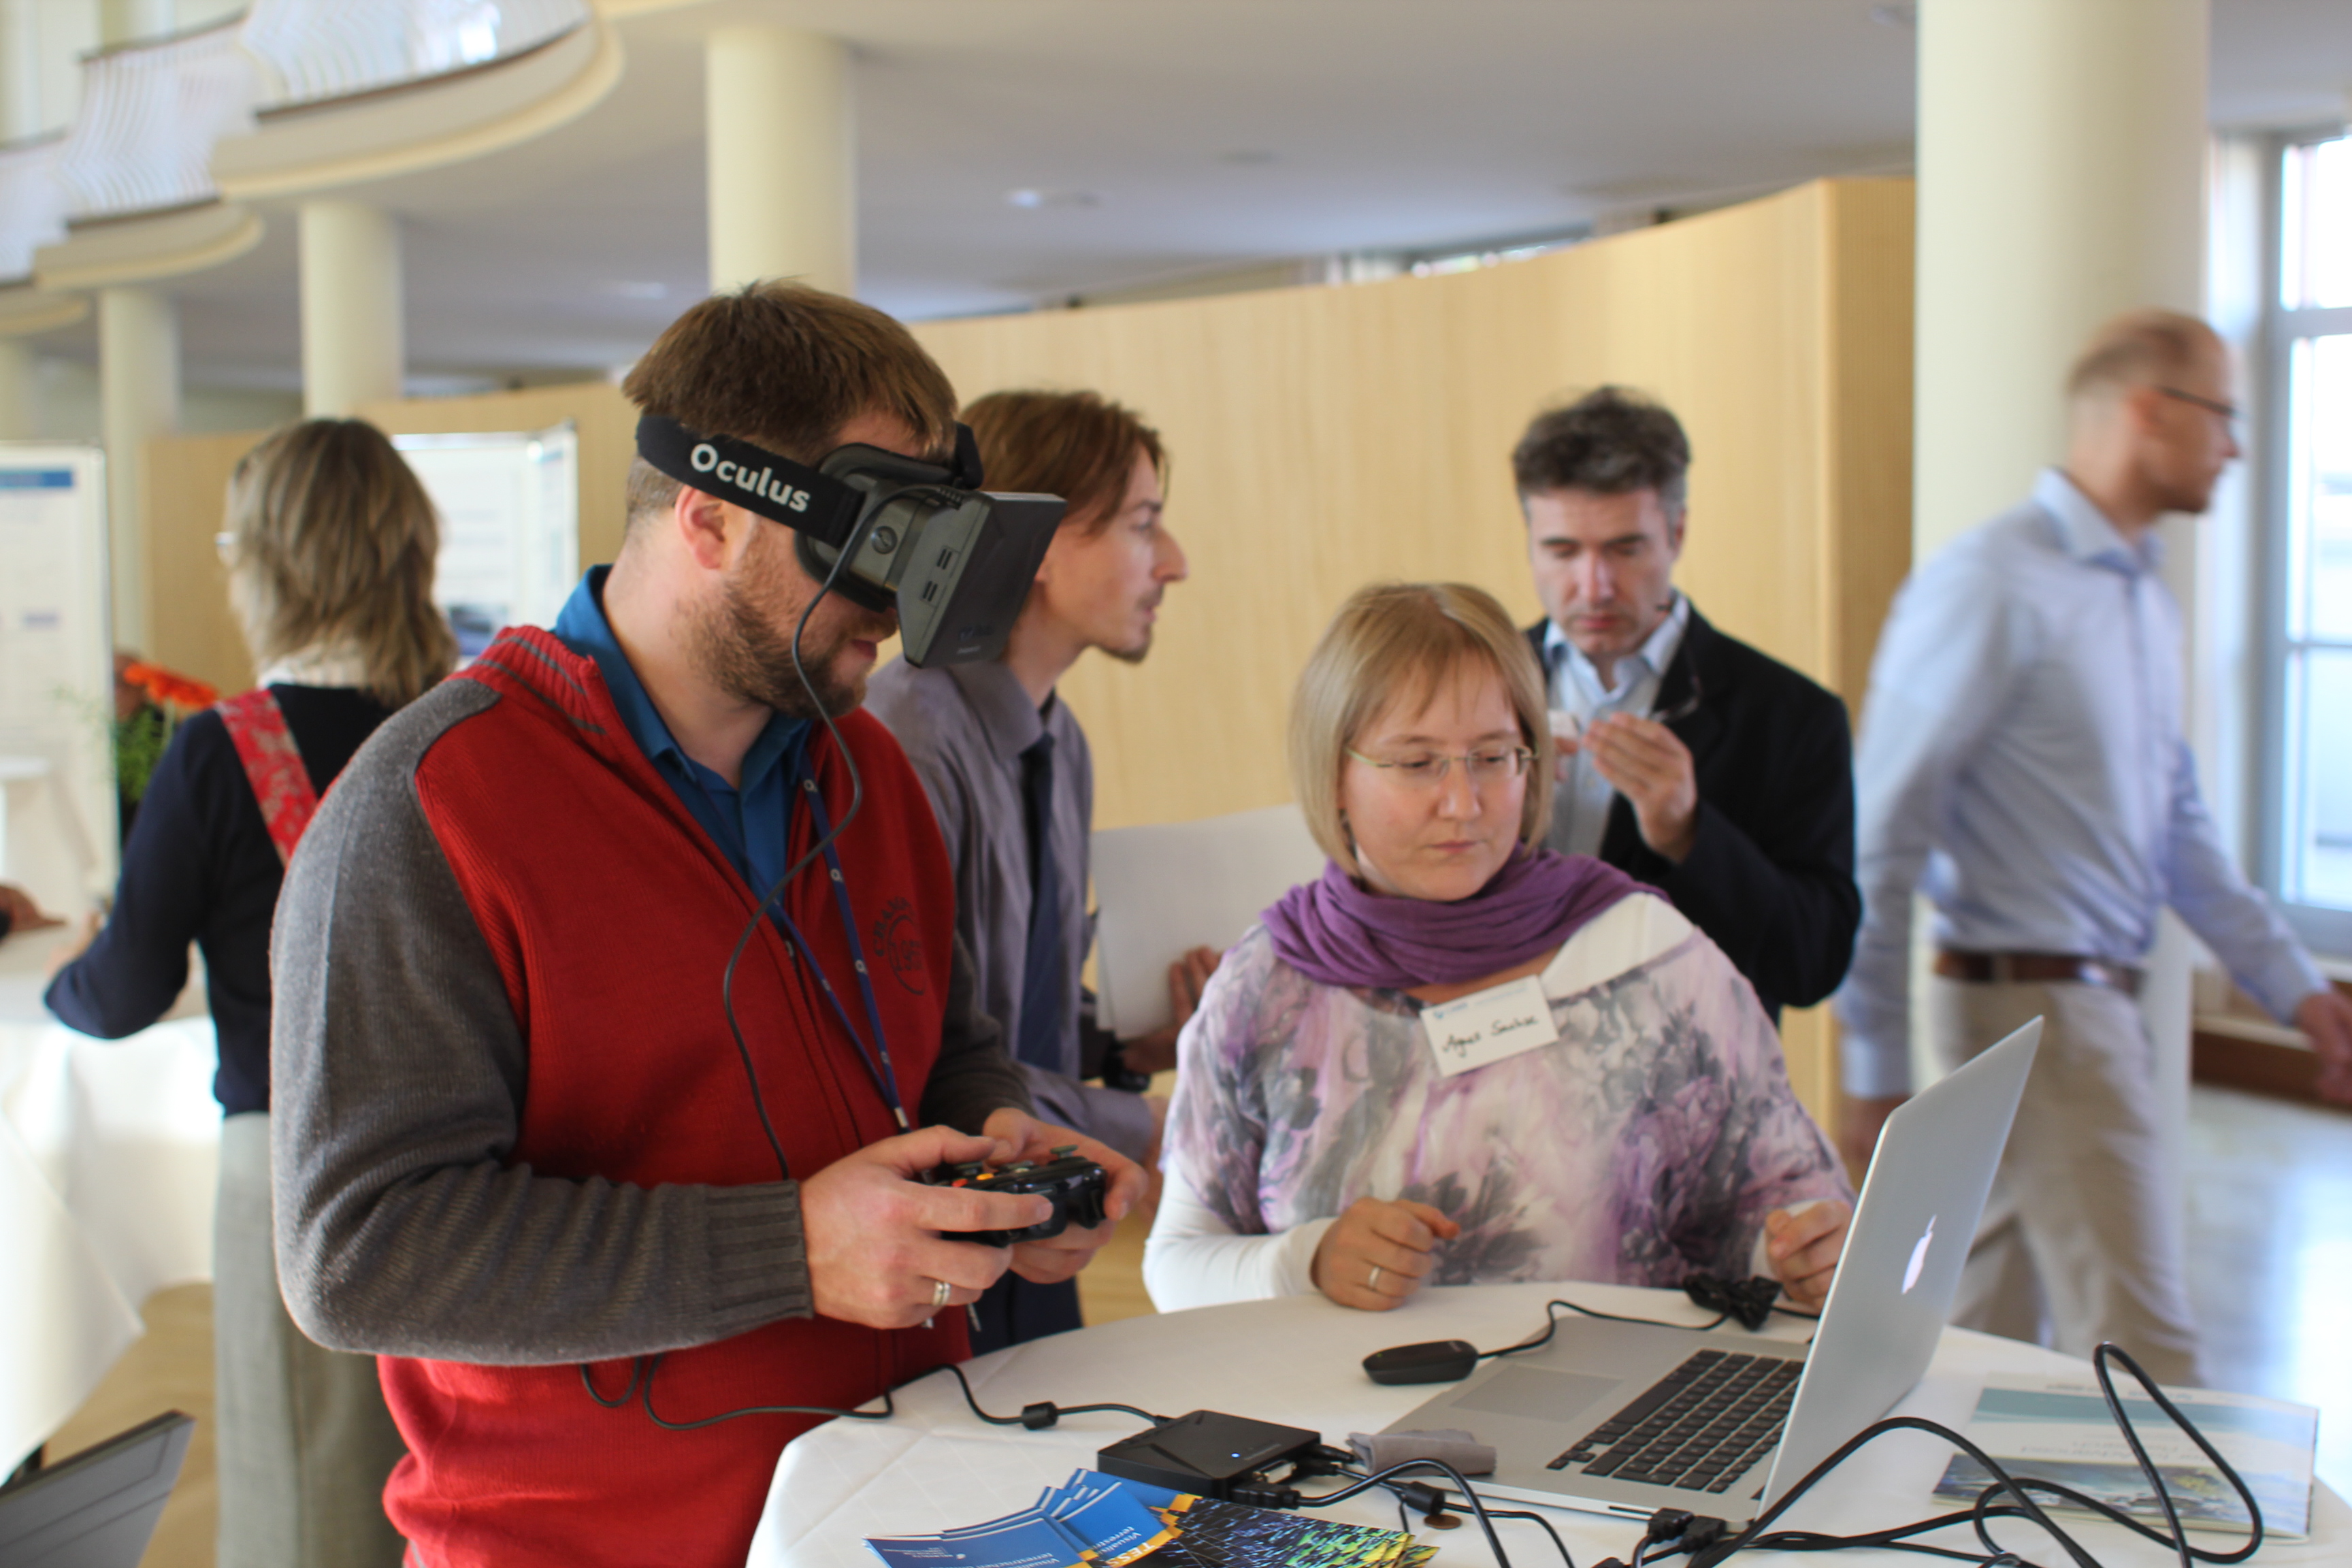
\includegraphics[width=\linewidth]{images/rift.jpg}
\caption{Mobile presentation at a scientific conference}
\label{fig:rift}
\end{figure}

\subsection{Software}
\label{software}

Because of the clustered setup we can only use software which can run in parallel and synchronizes the current state across all involved machines. There are specialized software with integrate cluster rendering capabilities and middleware software which add this functionality on top of non-clustered applications. These middlewares intercept graphic commands from a desktop application and redistribute them to a render cluster such as Techviz~\cite{web:techviz} or Conduit~\cite{web:conduit}. Such middleware software products allow to run a regular 3D desktop application in a VR environment with stereoscopy and tracking enabled. A data conversion is not necessary for this setup but interaction and presentation techniques are limited by the desktop application employed and performance is lost during graphic commands interception and distribution to the cluster such that immersion and feedback are severely affected.

For presenting visualizations we use the software packages with native cluster rendering capabilities such as \emph{VRED}, \emph{ParaView} or \emph{Unity} in conjunction with \emph{MiddleVR}. All of these are introduced in the following:

\paragraph{\emph{VRED}}
is a commercial software by \emph{Autodesk} (former \emph{PI-VR}) specialized in photorealistic real-time product rendering running on Windows~\cite{web:vred}. It is build on top of \emph{OpenSG}, an open-source scene graph library which offers clustered rendering~\cite{opensg}. \emph{VRED} can arrange imported 3D objects in a virtual scene, allows for tweaking of material (properties how the surface of the 3D objects reacts to lighting ) and lighting parameters but is neither a modeling software nor are there many interaction possibilities besides viewer movement and object selection. It has a plug-in interface but no documentation is available from \emph{Autodesk} on how to address it. An advantage of the software is that \emph{VRED}'s editor can be directly connected to the \emph{VISLab}'s display so that local changes to the scene done at the presentation terminal are visible immediately on the video wall.

\paragraph{\emph{ParaView}}
is an open-source data analysis and visualization software~\cite{paraview} by \emph{Kitware Inc.} build on top of the \emph{Visualization Toolkit}~\cite{vtk} (\emph{VTK}). Both technologies are also integrated in our visualization workflows (see \ref{workflows}). \emph{ParaView} allows to quickly create visualizations and implements a large number of well established visualization algorithms and techniques. It can run on distributed memory architectures to analyze large datasets and to drive VR displays. Using \emph{ParaView}, we can modify visualization parameters directly in the VR environment. Unfortunately, it lacks more sophisticated interaction and presentation features.

\paragraph{\emph{Unity}}
is a complete game engine by \emph{Unity Technologies}~\cite{goldstone:unity3d}. It is available in a free and a commercial editor variant with the latter supporting more advanced rendering techniques (soft shadows, HDR, post-processing effects) and team collaboration features. \emph{Unity} has several rendering backends (\emph{OpenGL}, \emph{OpenGL ES}, \emph{DirectX}) so it can be run on all major platforms as well as on the Web (with an additional browser plug-in)~\cite{web:unity}. \emph{Unity}'s basic scope of operation does not include any interaction functionality but it has a comprehensive scripting documentation and a vivid plugin community so that it is very easy to integrate missing features. Application testing can be done directly in the \emph{Unity} editor by tweaking the application at runtime. However, \emph{Unity} created applications cannot run in a clustered environment. Therefore \emph{MiddleVR} is used.

\paragraph{MiddleVR}
is a generic virtual reality middleware from \emph{i'm in VR} designed to work with different 3D applications~\cite{web:middlevr}. It features a graphical configuration tool to setup VR systems independent of specific software. It implements interaction devices, stereoscopic rendering and clustering when using software not supporting this functionality. The \emph{MiddleVR} configuration is then used in a \emph{Unity} plugin to enable all these features in Unity applications. The \emph{MiddleVR}-enabled Unity application is VR system agnostic, once compiled it can be run on any VR system supported by \emph{MiddleVR}. A disadvantage of this approach is that the final application cannot be run inside the Unity editor but stand-alone, so that it cannot be altered interactively at runtime. The fact that a recompilation of the application takes just a few seconds weakens that drawback.

For the future, we will focus on the use of Unity as a platform for highly interactive visualizations to illustrate and discuss complex phenomena. In contrast, ParaView is more suited for rapid prototyping and exploration of complex datasets.

\subsection{Workflows}
\label{workflows}

For simulation we employ \emph{OpenGeoSys}~\cite{kolditz:ogs}, an open-source platform and flexible numerical framework for the simulation of thermo-hydro-mechanical/chemical processes in porous and fractured media with applications in geoscience and hydrology. In order to simulate these processes models are defined that include as much relevant data as possible to account for all phenomena defining that natural system. Heterogeneous datasets representing the model characteristics are given as input parameters to the simulation software which returns result datasets predicting system behavior in areas of interests.

We are both using visualization when setting up the model and simulation as well as to analyze simulation result data. As a basis for creating visualizations we employ \emph{VTK} which is also integrated into the \emph{OGS Data Explorer} framework~\cite{rink:eesenvirvis} as well as \emph{ParaView}.

We provide utilities and \emph{ParaView} plugins to convert \emph{VTK} visualization data to formats supported by the VR frameworks used in the \emph{VISLab}, i.e. OpenSG for \emph{VRED}~\cite{bilke:vtkosgconverter} and Autodesk FBX for Unity~\cite{bilke:vtkfbxconverter}. Conversion can be either done manually in the \emph{OGS Data Explorer} or in a batch process by employing \emph{ParaView}'s Python scripting interface. The second approach is especially useful when converting large sequences of complex datasets such as time steps of simulation results from transient finite element models. During conversion, meta data is appended to the datasets to include information not necessarily supported in FBX such as a specific material and rendering setup or time stepping information. This meta data is evaluated when loading the datasets into Unity and can be queried, i.e.~for displaying the time stepping information as a text overlay. Multiple datasets can be arranged both in a spatial but also in a temporal context and a variety of presentation techniques (i.e. defining camera animations, fading in/out of datasets, selection of subsets, displaying additional information), see~\cite{rink:eesenvirvis} for details.

\section{Overview of VISLab Applications}
\label{overview-of-VISLab-applications}

\myedit{}{Ich w\"urde die Subsection-\"Uberschriften weglassen (die sind ohnehin sehr willk\"urlich) und die Subsubsections zu Subsections machen. Du kannst das ganze ja trotzdem sinnvoll anordnen, so dass das thematisch einen fliessenden �bergang gibt\dots}

\subsection{Hydrology and Climate}
\label{hydrology-and-climate}

The challenge for visualization in hydrology and climate research is the integration of a large variety of heterogeneous data from different sources at multiple spatial and temporal scales (Rink et al. 2012).


\subsubsection{Ammer Catchment}
\label{ammer-catchment}
% KR: Ich wuerde Ammer *vor* Western Dead Sea erklaeren, weil beides steady-state GW-models sind, aber die Ammer-Geschichte "einfacher" ist, d.h. bei WDS kommen zumindestest einige Dinge hinzu, so dass man es besser rechtfertigen kann, dass beide Modelle hier im Paper erklaert werden.

The catchment of the river Ammer in southwest Germany has been selected as the study region for a holistic analysis of the water cycle coupled to reactive solute transport,  for addressing water and solute fluxes at the catchment scale as a function of and in feedback with changes in climate, land use, and water usage~\cite{grathwohl:wessti}. The river has a length of 25\,km and is a tributary to the Neckar. Its catchment has a size of 180\,km\textsuperscript{2} with a geology comprised of a sequence of Triassic strata forming a landscape characterised by escarpments~\cite{selle:wessti}. The Ammer is mainly fed by groundwater from the karstic and fractured aquifers and drains the catchment at a rate of ca. $1\,m^3/s$.

The finite-element groundwater model is based a digital elevation model with a resolution of 100\,m in combination with interpolated subsurface layers based on the stratigraphic data of over $100$ boreholes. For simulation purposes, the subsurface information has been combined into four separate layers, consisting of a partly karstified limestone aquifer overlaid by Keuper-layers. In addition, the scene includes the stream network and groundwater production wells, which are employed as boundary conditions for the model as well as raster data with groundwater recharge information. Based on the results of a steady-state groundwater recharge simulation, the presentation also includes iso-surfaces representing the groundwater head as well as stream tracers for the visualisation of flow paths within the catchment. See Selle et al~\cite{selle:wessti} for more information on the groundwater study and Rink et al~\cite{rink:wessti} for model setup and data visualization.

\subsubsection{Western Dead Sea - Sustainable Management of Water in Arid and Semi-Arid
Regions}
\label{western-dead-sea---sustainable-management-of-water-in-arid-and-semi-arid-regions}

Agnes Sachse \cite{graebe:modelcare}

\subsubsection{Climate Data}
\label{climate-data}

Carolin Helbig

\myedit{}{Sowas in der Art sollte bei dir in der Introduction stehen und dann hier nicht nochmal auftauchen. Daf\"ur fehlen hier noch ein/zwei S\"atze, was das \"uberhaupt f\"ur eine case study ist, warum die gemacht wurde, etc.)} Figure \ref{fig:wind} shows an example of a subset of a simulation domain, where we concurrently visualized wind field, mass fraction, humidity and heat fluxes in relation to the digital elevation model. The visualization is used to provide a detailed look at processes \myedit{}{(welche?)} and investigate if they have been captured correctly by the model. With the help of animation, the different time steps are displayed and the user can analyze the development of convection and observe heat transports, for instance. The challenge of these datasets is their highly multivariate character that requires stereoscopic 3D visualization for analysis. The visual combination of simulation, observation, and statical data, which differ in their spatial and temporal resolution, supports the scientists to verify, falsify and generate their hypothesis~\cite{helbig:eesenvirvis}.

\begin{figure}
  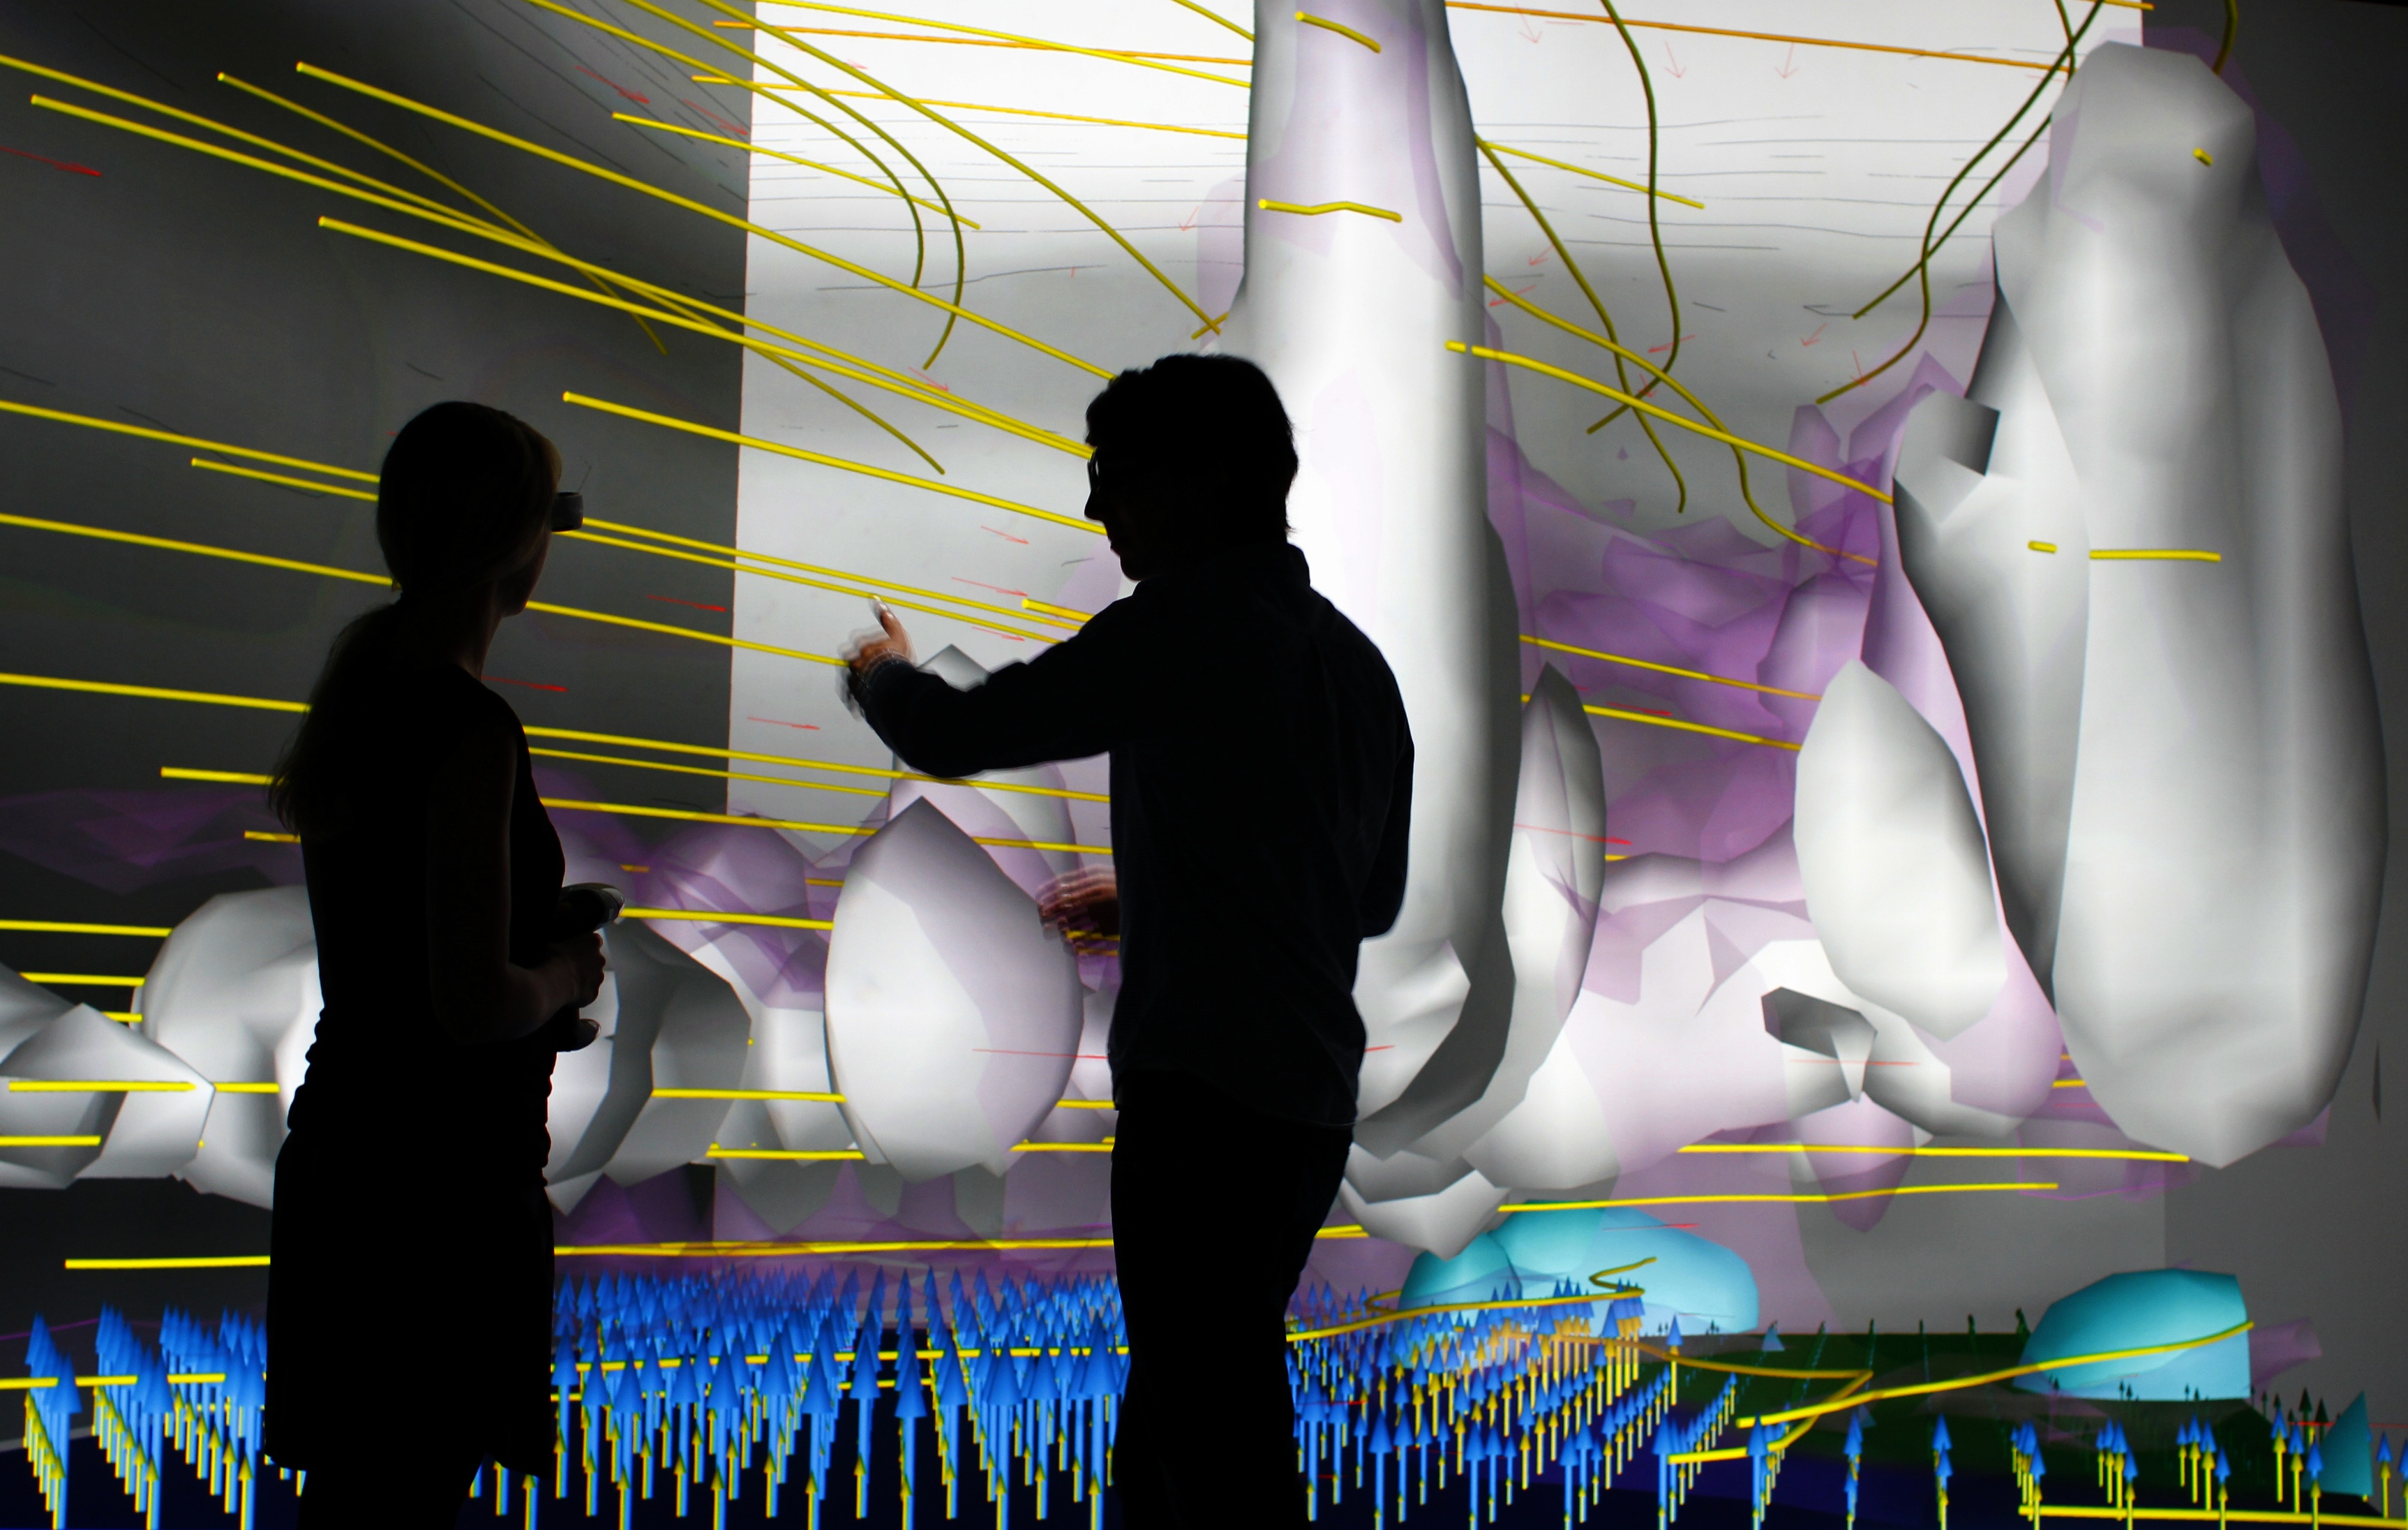
\includegraphics[width=\linewidth]{images/wind.jpg}
  \caption{Climate simulation data visualization showing wind fields (streamlines), mass fraction (white and blue isosurfaces), humidity (slices in the back) and heat fluxes (arrow glyphs on the surface) above the digital elevation model.}
\label{fig:wind}
\end{figure}

\subsubsection{Pore-Scale}
\label{pore-scale}

Dmitry Naumov

\subsubsection{Nankou}
\label{nankou}

Feng Sun \cite{sun:ees}

\begin{figure}
  \includegraphics[width=\linewidth]{images/nankou.jpg}
\caption{TODO Nankou groundwater deteriation}
\label{fig:nankou}
\end{figure}

\subsubsection{Oman - Saltwater Intrusion}
\label{oman---saltwater-intrusion}

Marc Walther

\begin{figure}
  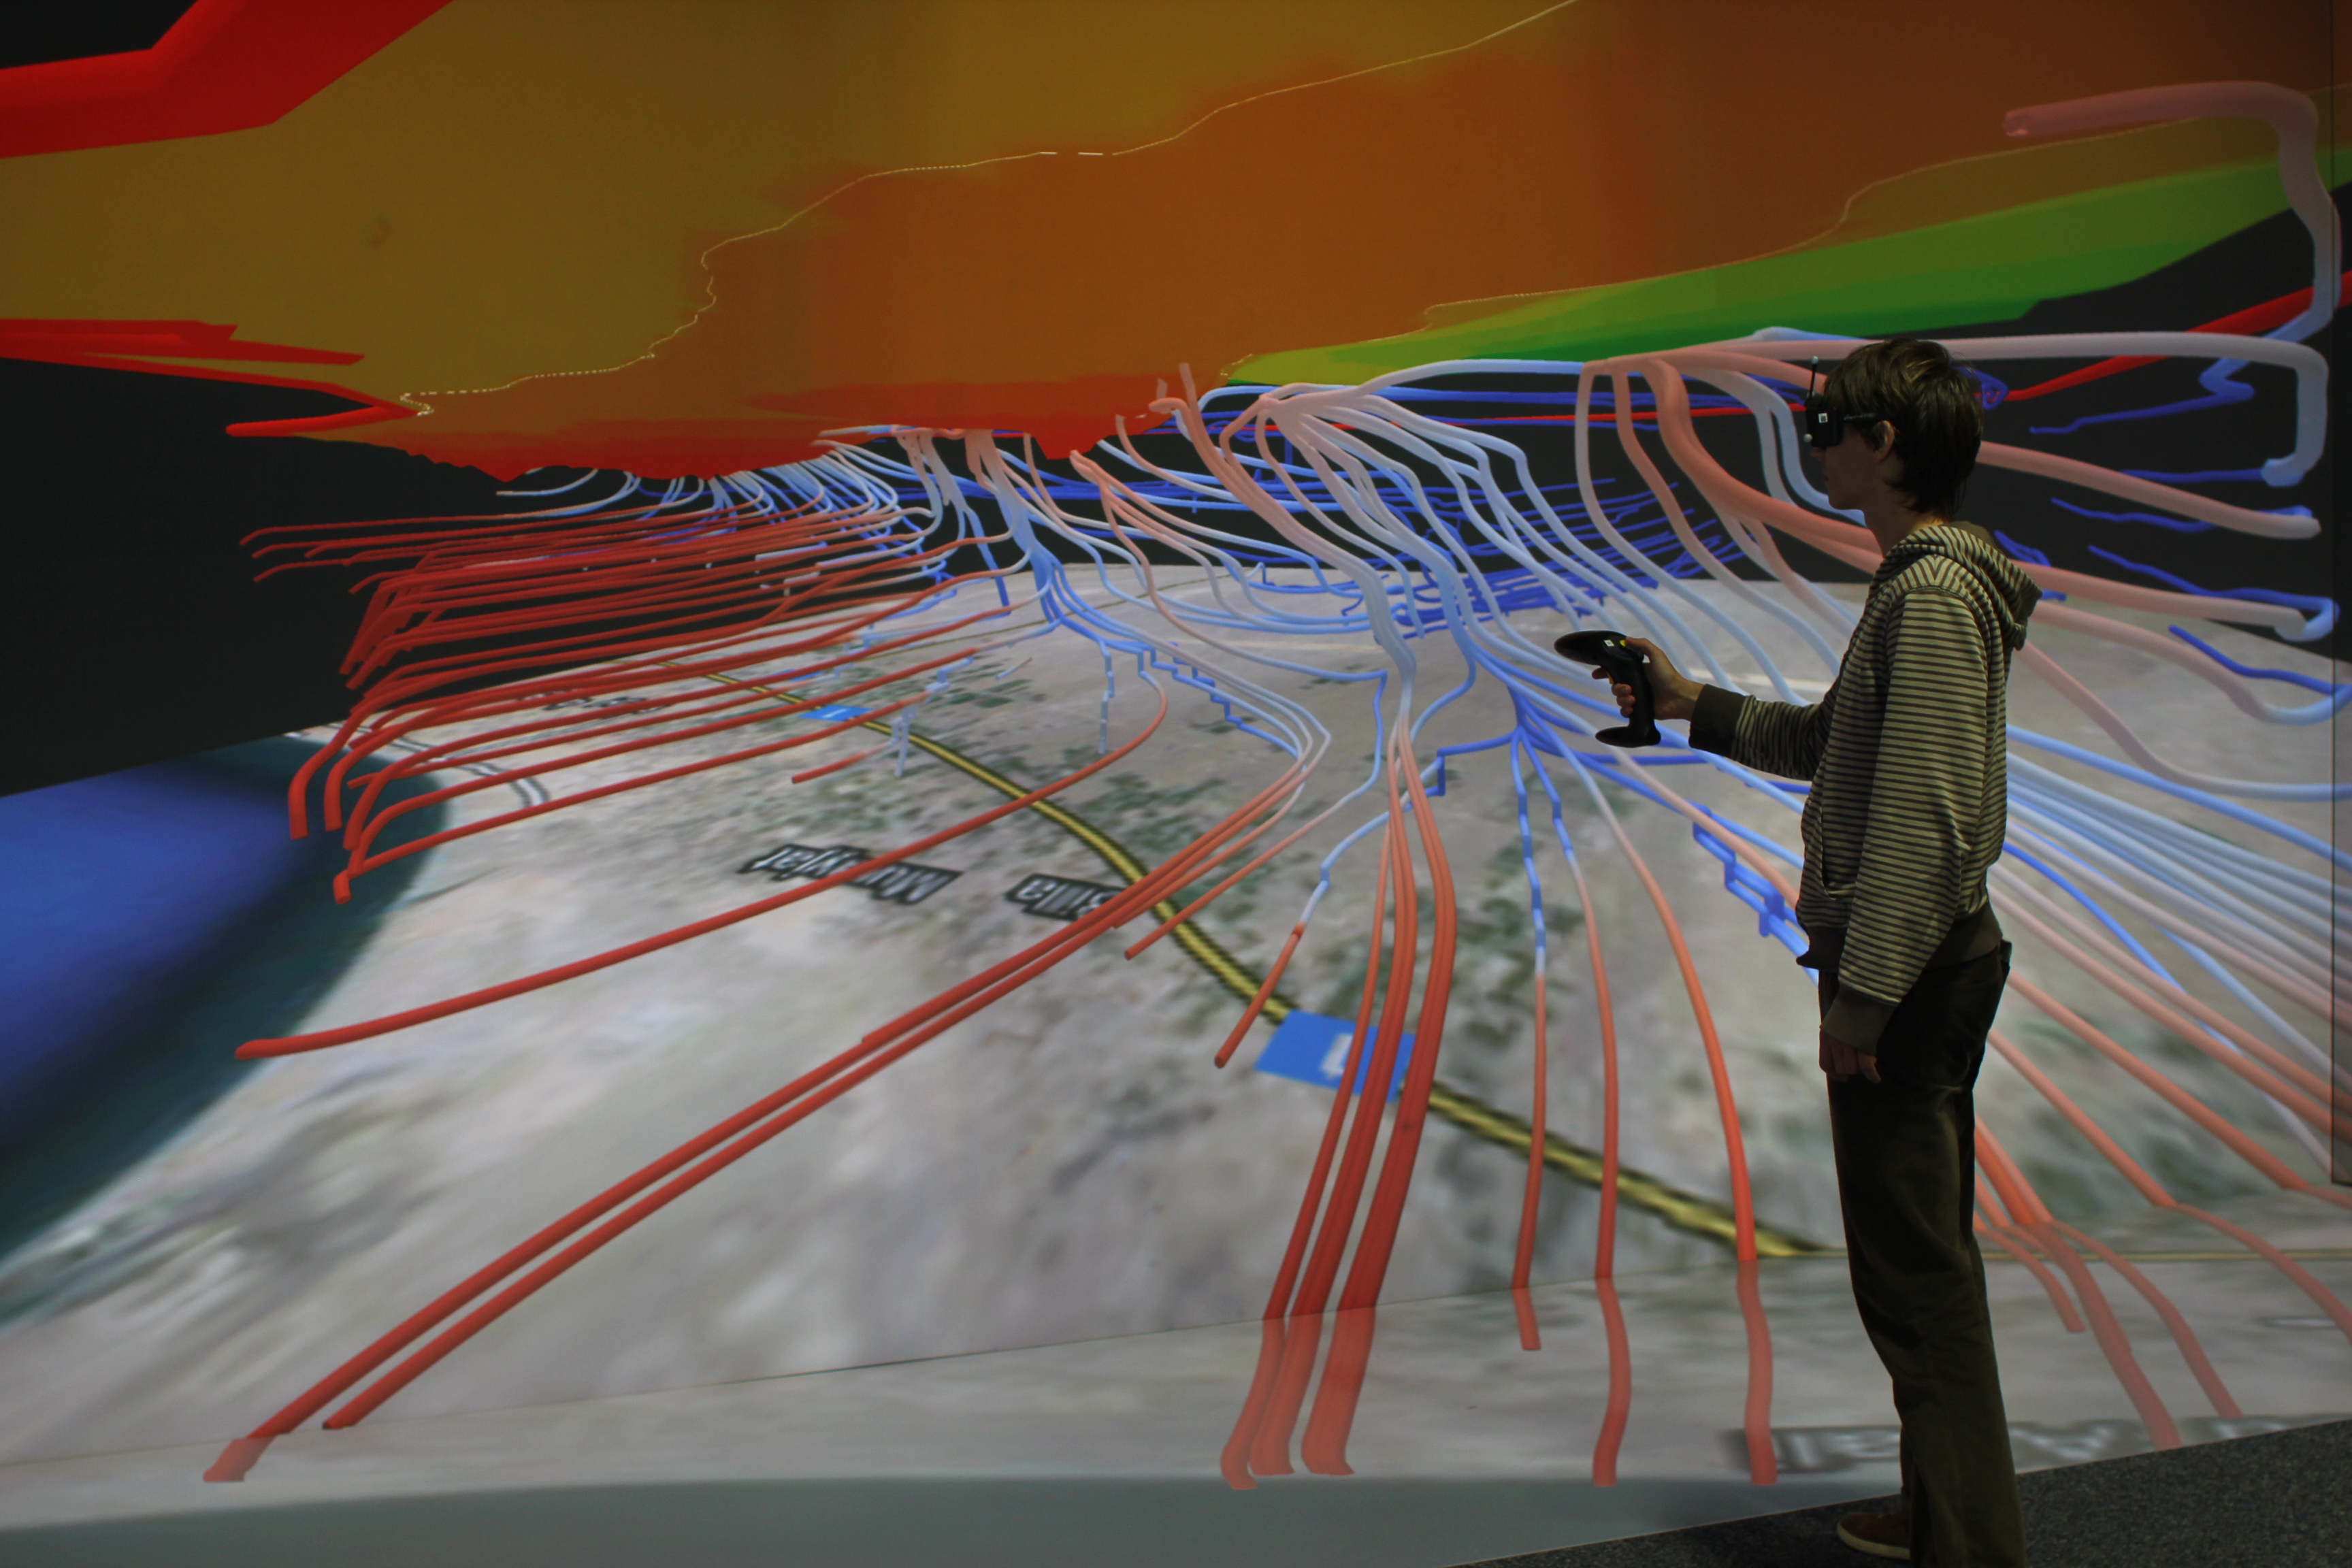
\includegraphics[width=\linewidth]{images/oman.jpg}
\caption{TODO}
\label{fig:oman}
\end{figure}

\myedit{}{(Das geh\"ort hier alles nicht rein. Wenn schon allg. Bla-bla, dann lieber irgendwas zu Wassermanagement in ariden Gebieten oder so.)} One of these case studies, a region scale study on density driven flow in a coastal aquifer that is used as source for agriculture irrigation, intensively made use of visualization options during model setup, verification of the variable density process, and for the transfer of knowledge to local authorities~\cite{walther:cam, walther:eesenvirvis}. Firstly, visualization was used to investigate plausibility of the set up hydro-geological model, that was constructed based on an extended inverse weighting distance interpolation~\cite{walther:modelcare}. Secondly, large datasets of model calibration and long term scenario simulations of the saltwater intrusion process were analyzed by utilizing \emph{ParaView}. \emph{ParaView} was run on a parallel cluster computer to omit bandwidth limitations to copy large data and to reduce computational burden on standard desktop machines. Thirdly, results of the modeling were visualized, which helped during discussions with experts and tremendously aided in knowledge transfer during a visit of Omani authorities from the Ministry of Regional Municipalities and Water Resources. Additionally, throughout all states of model development, calibration, scenario analysis, and result presentation, the \emph{VISLab} was utilized~\cite{walther:eesenvirvis}.

\subsubsection{TERENO-Observatory Harz/Central German Lowlands}\label{tereno-bode}

TERENO is a large-scale project aims to catalogue the longterm ecological, social and economic impact of global change at regional level~\cite{zacharias:tereno}. Four areas in Germany have been selected and are now heavily instrumented to allow extensive studies and simulations for researchers from different disciplines. Hydrogeological analysis in central Germany is being conducted in the catchment of the River Bode with a size of 3,100\,km\textsuperscript{2}. Within that area a number of intensive test sites have been selected, ranging in size from a small area of about one hectare, concerned with assessment of water balance in a forested region, to the complete catchment of one of the Bode's tributaries with a size of over 450\,km\textsuperscript{2} where hydrological processes in the stream as well as in the hyporheic zone are investigated~\cite{schmidt:selke, trauth:flow}.

The presentation consists of over $70$ heterogeneous data sets of different scale and resolution. Most notable are surface representations, consisting of a terrain model of the whole region with over 1 mio triangles with a max edge length of 30\,m. Terrain models of the intensive test sites also exist at a much finer resolution, ranging from 30\,m for the larger regions to just 1\,m for the regions covering 1\,km\textsuperscript{2} or less. Various colour transfer functions or textures can be applied to these surfaces, including elevation information, soil moisture, or indication of land use. While textures are originating from raster data, transfer functions are based on statistical data or look-up tables. Geometrical information includes the courses of streams at various resolutions and displayed with different prominence. Furthermore, the scene includes climate stations, measurement networks, bathymetries of some of the larger water bodies within the region, structural models for the subsurface of two intensive test sites, borehole data and much more. Most regional data sets are only visible when the presentation zooms in on the intensive test site they are located in, to avoid unnecessary clutter of the overall scene. Still, data integration of so many data sets acquired by different means is quite challenging a number of different preprocessing steps were required for concurrent display and visibility of small data sets within the larger context~\cite{rink:wessti, rink:eesenvirvis}.

\subsubsection{Saudi-Arabia - Groundwater
Flow}\label{saudi-arabia---groundwater-flow}

Thomas Kalbacher \cite{zehner:modelcare, rink:iwas}

\subsubsection{Streambed}\label{streambed}

Nico Trauth

\begin{figure}
  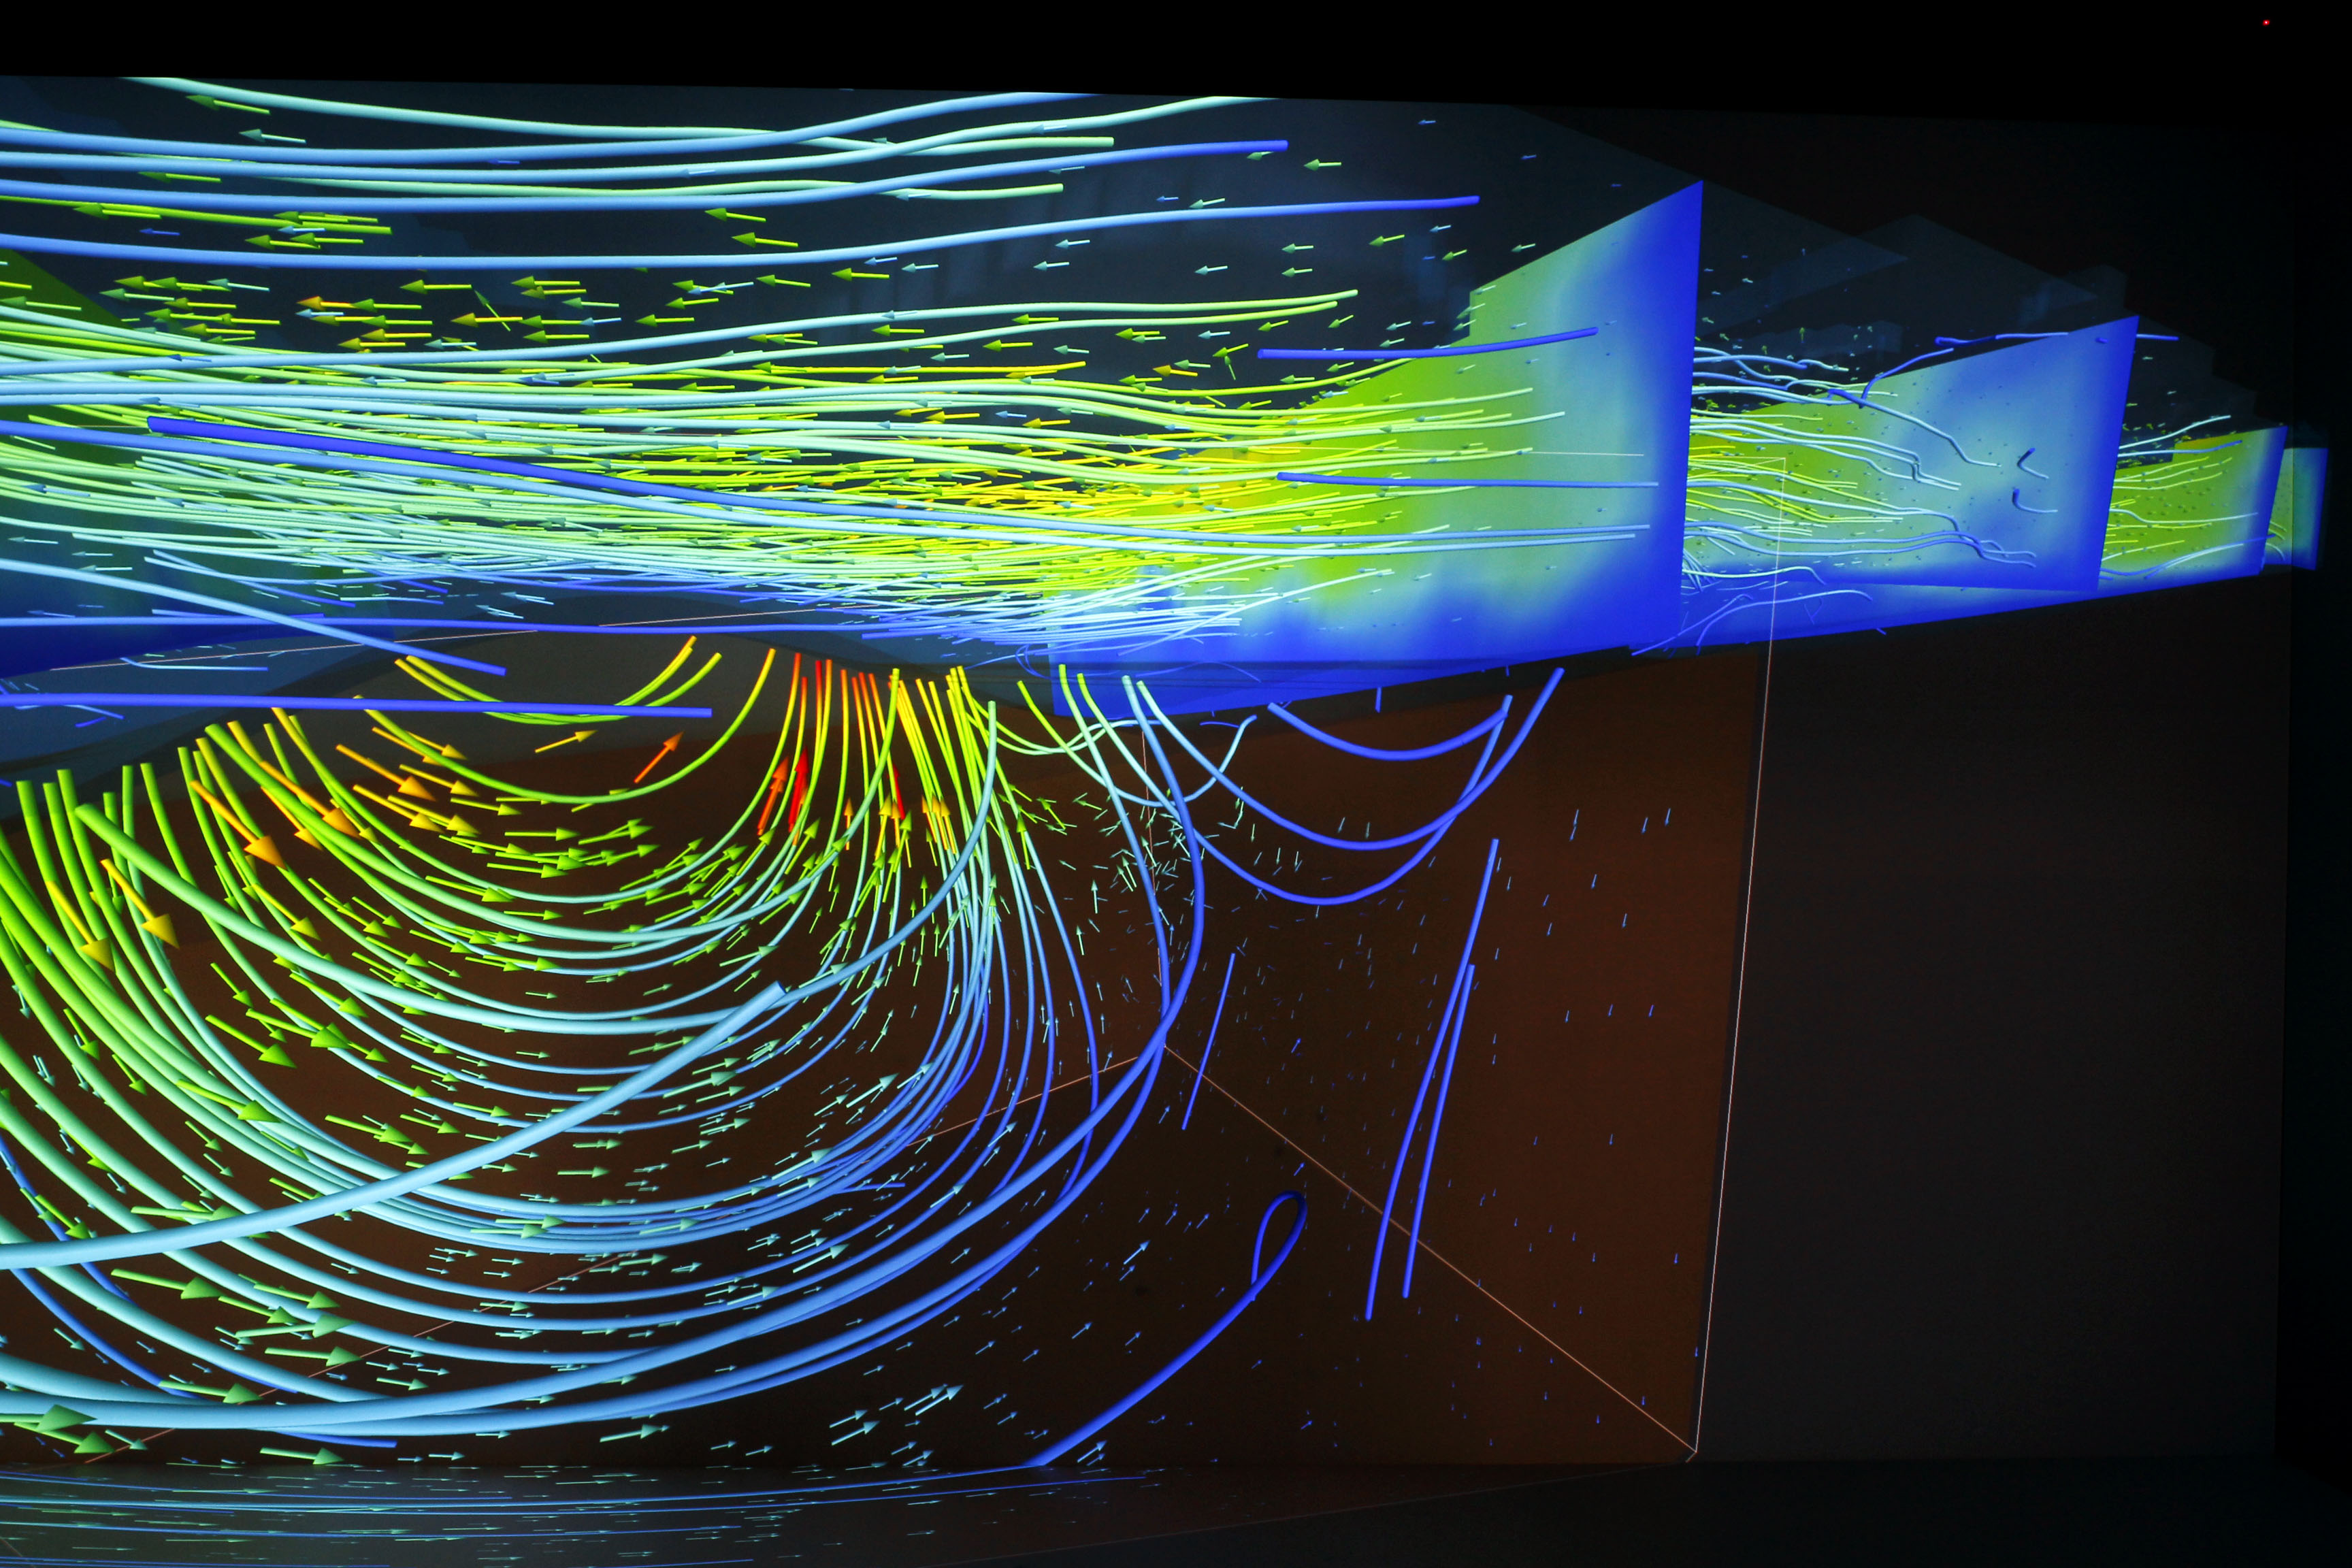
\includegraphics[width=\linewidth]{images/streambed.jpg}
\caption{TODO}
\label{fig:streambed}
\end{figure}

\subsection{Geosciences and Energy}\label{geosciences-and-energy}

In geosciences we have to deal with complex geological structures containing different architectural elements such as layers, faults, diapirs, fracture networks. Thermo-hydro-mechanical-chemical processes under extreme thermodynamic conditions have to be considered for utilizing geological reservoirs, e.g.~for geothermal energy (Zehner et al. 2010).

\subsubsection{Gro{\ss}-Sch\"onebeck - Geothermal Energy}
\label{grouss-schoenebeck---geothermal-energy}

Norihiro Watanabe

\subsubsection{Otway-Basin - CO2-Storage}
\label{otway-basin---co2-storage}

Jennifer Ziesch

A data conversion tool for seismic data was developed~\cite{bilke:simpleseismicreader} which allows to import rectilinear-shaped seismic data in a plain text format into \emph{ParaView} via its plugin-interface. This is necessary because typically SEG-Y formated seismic dataset does not allow an immediate interactive visualization. \emph{OpendTect}~\cite{web:opendtect} was used to transform the seismic data of the Otway Basin (available in SEG-Y format) to a plain text data format which can then be easily processed by our tool. In ParaView the seismic data gets imported as universal 3D image data.

\begin{figure}
  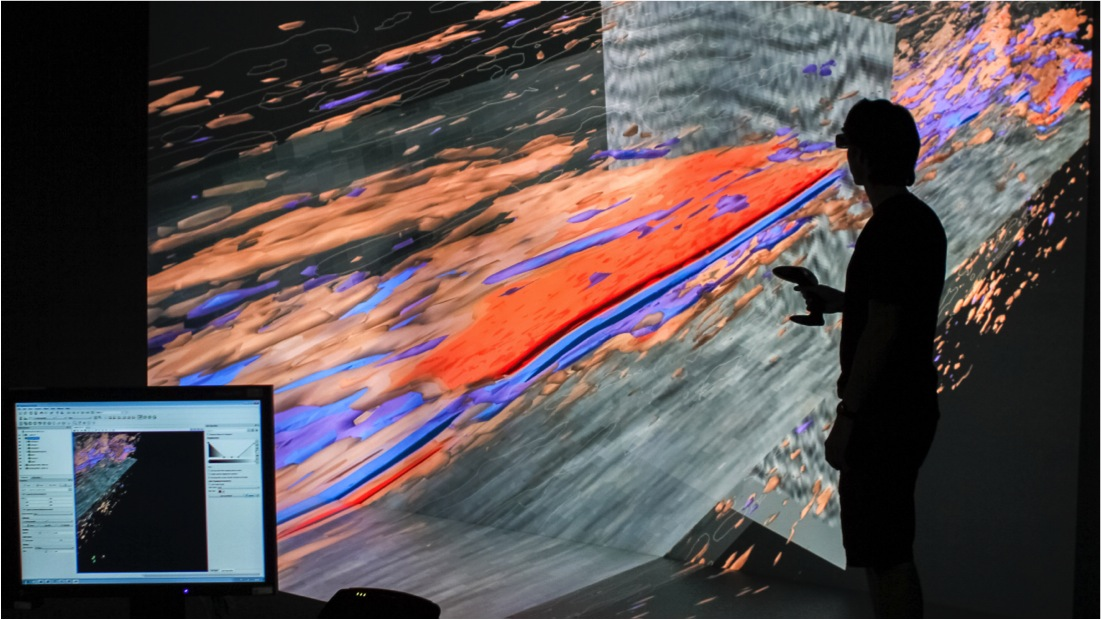
\includegraphics[width=\linewidth]{images/seismic.jpg}
\caption{ParaView running in the VISLab showing a spatial subset and cross-sections of 3D seismic data and isosurfaces of interesting features.}
\label{fig:seismic}
\end{figure}

\subsubsection{Thuringia Basin - Faults}
\label{thuringia-basin---faults}

Thomas Fischer, Dmitry Naumov

\subsection{Landscape and Biodiversity}
\label{landscape-and-biodiversity}

\myedit{}{Die \"Uberschrift w\"urde ich wieder rausnehmen. Den untenstehenden Satz kannst du trotzdem nutzen, um auf eine andere Gruppe von Case Studies \"uberzuleiten.}

Many man-made actions have an impact on landscapes as well as to biodiversity surrounding us and this should be communicated to and discussed with the public, so that people are aware of this fact. Virtual Environments are very well suited for the integration and visualization of various data within a unique geographic context for discussion and decision making of different options (TODO Zehner 2010).

\subsubsection{Biodiversity in Rain Forests}
\label{biodiversity-in-rain-forests}

Andreas Huth Formind \cite{kohler:98}

\begin{figure}
  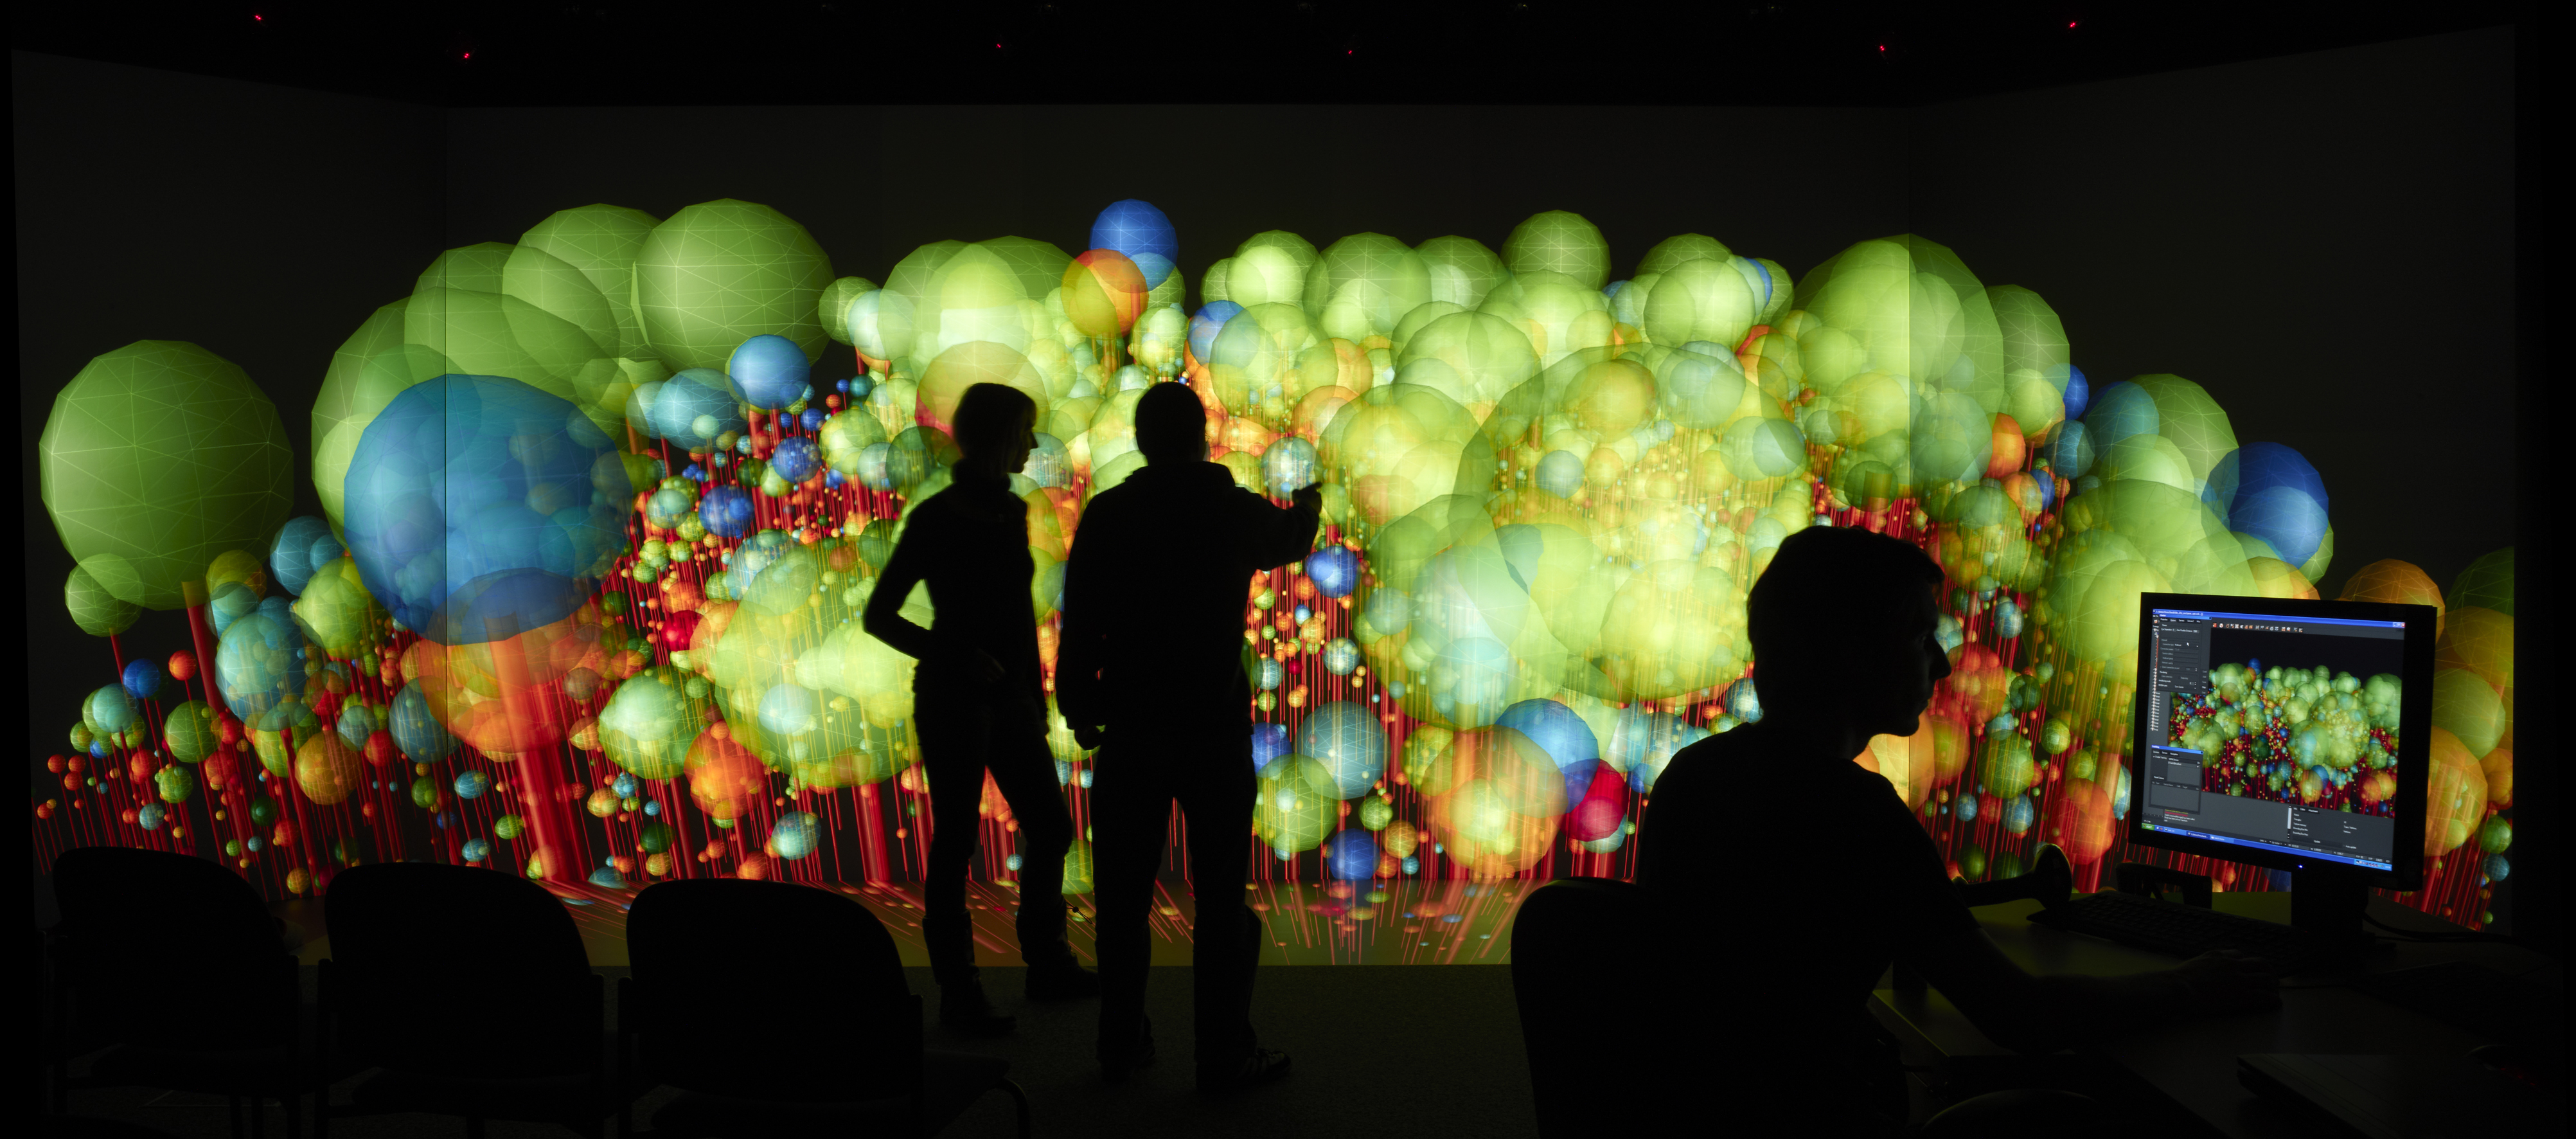
\includegraphics[width=\linewidth]{images/biodiversity.jpg}
\caption{TODO}
\label{fig:biodiversity}
\end{figure}

\subsubsection{Windpark Planning}
\label{windpark-planning}

Bj\"orn Zehner

\subsection{Urban Environments}
\label{urban-environments}

Lars Bilke, TODO put on GitHub and DOI

To help in the creation of urban environment visualizations usable for social sciences and for urban development a procedural building model generator was developed~\cite{bilke:master,procedural:modelling}. The software called \emph{CityGenerator}~\cite{bilke:citygenerator} allows to procedurally generate building models as well as small city scenes out of simple building blocks such as fa\c{c}ade textures, doors, windows and decoration elements. The user can specify input parameters including the building footprint, building height and designs a template fa\c{c}ade in a graphical user interface. This template fa\c{c}ade is defined by a set of grammatic rules~\cite{procedural:buildings}. The actual model generation is implemented as a \emph{VRED}-plugin allowing for immediate presentation in the \emph{VISLab}. \emph{Level-of-detail} (LOD) techniques ensure a good performance of larger scenes.

\begin{figure}
  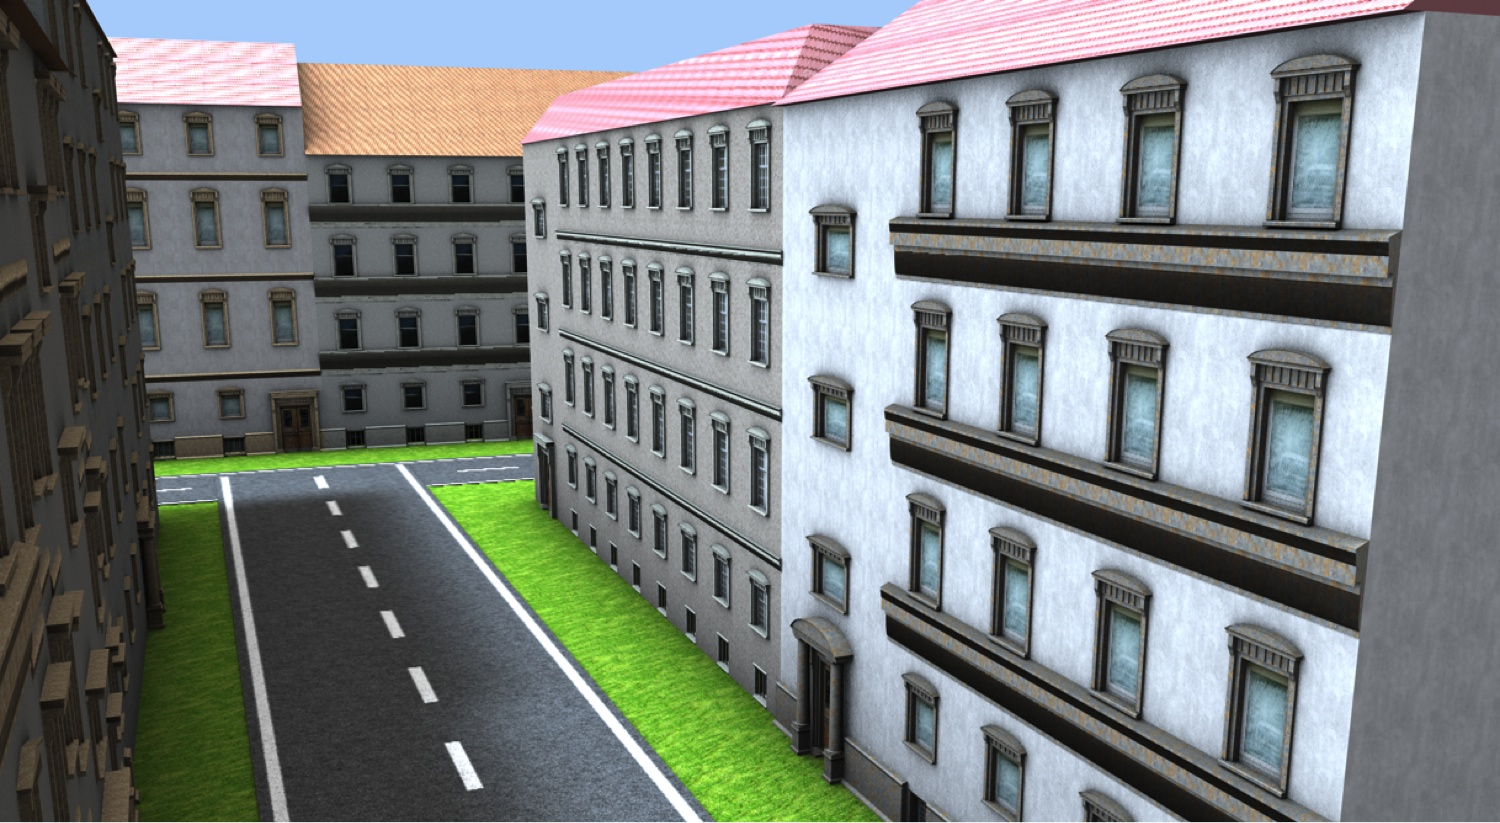
\includegraphics[width=\linewidth]{images/city.jpg}
\caption{TODO}
\label{fig:city}
\end{figure}

\section{Future work}
\label{future-work}

\myedit{}{(\"Uberarbeite die n\"achsten zwei S\"atze nochmal, die sind derzeit sehr vage, zusammenhanglos und teilweise irref\"uhrend.)}
For the future we would like to integrate new visualization techniques to better incorporate scientific visualization in the daily research work, especially into high-performance computing (HPC). To achieve these goals we will integrate visualization methods into simulation codes and simplify the technical setup to unlock more fields of applications.

\subsection{In-situ visualization}
\label{in-situ-visualization}

In-situ or Co-visualization allows to create result analysis and visualization as a part of the simulation process. \myedit{}{(Wieder so ein Sprung, die beiden S\"atze haben nix miteinander zu tun.)} HPC systems are getting more processing power, more memory and more communication bandwidth every year. But not all of these capacities are growing at an equal rate. Especially communication bandwidth can be the limiting factor in various applications.

Normally the simulation process is tripartite:\myedit{}{(Das stimmt imo nicht ganz, es sollten vier Teile sein: Pre-proc, model setup, simulation, post-proc)} in the \emph{preprocessing} \myedit{part,} the model of the simulation gets defined and all input data gets prepared for the simulation run. Typically the \emph{simulation} step produces large amounts of result data \myedit{(Das ist wieder sehr unspecifisch. Das m�sste man ausf�hrlicher schreiben, am besten mit ein paar buzz-words wie transient, coupled, multi-parameter, etc.)} which are then processed and analyzed in the \emph{postprocessing} step \myedit{(Auch wieder nur so halbrichtig\dots die Daten werden ja nicht einfach prozessiert, sondern man wendet ja gezielt Filter/Transformationen an, um die interessanten Aspekte sichtbar zu machen.)}. Usually the postprocessing takes place on frontend-nodes of the HPC system or on the users machine and storage capacity may be limited. In the latter case all result data have to be transfered over the computer network. The analysed data as the outcome of the postprocessing step can be much smaller than the simulation result data. Therefore the postprocessing should become integrated into the simulation itself to avoid the communication bottleneck and to transfer the analyzed data only.

\myedit{}{(Meine Argumentation w\"are eher, dass man schon zur Simulationszeit sehen will, ob sich der Prozess plausibel entwickelt. Daf\"ur kann man eine processing-pipeline definieren, die auf jeden Ausgabeschritt die gleichen (Filter-)Methoden anwendet, so dass man instant das Ergebnis sieht, das einen interessiert. So ungef\"ahr, was du im n\"achsten Abschnitt beschreibst, aber mit ein paar einf\"uhrenden S\"atzen und etwas ausf\"uhrlicher.)}

We will use the library \emph{Catalyst}~\cite{web:catalyst} for integration of such an in-situ visualization into \emph{OpenGeoSys}. \emph{Catalyst} is an extension of \emph{VTK} / \emph{ParaView}. On the basis of a representative example dataset the user defines a visualization pipeline (either by a script or interactively in \emph{ParaView}) which is then executed after defined time step intervals of the simulation. During simulation time the user gets processed data as a result of the visualization pipeline, images of the visualization and an interactive remote visualization in \emph{ParaView}.

Furthermore it should be possible to view the live visualization in the VR environment of the \emph{VISLab} which is also connected to the EVE HPC system of the UFZ. \myedit{}{(Wenn du auf EVE verweisst, brauchst du entweder eine Quelle oder musst erkl\"aren, was das ist. Du k\"onntest auch nur allg. etwas von einem computing cluster schreiben. Das UFZ wird hier auch erstmalig erw\"ahnt, das willst du vielleicht auch entweder eher schonmal machen (Intro) oder ganz weglassen.)}

\myedit{}{(Das folgende w\"urde ich auf jeden Fall als Motivation f\"ur das ganze in-situ Zeugs vorziehen!)}
By observing the simulation process it is possible to detect errors in the input data early. The user can then cancel the simulation, adapt the input data and restart the simulation. This saves computational time and the decreases the workload of scientists and \myedit{}{(Das folgende versteh ich wieder nicht)} to an effective iterative process of refining and adapting the simulation. Because the in-situ visualization can be run without user interaction, it is also useful for software quality management and benchmarking\myedit{}{(Quelle?)}. Comparing visualization output and analyzed data between different program versions can be very helpful to detect errors in the code. \myedit{}{(oder in der Simulation!)}

\subsection{Simplified hardware setup}
\label{simplified-hardware-setup}

Our current hardware setup limits the usable 3D applications to software which can be run in parallel and synchronized on a computer cluster. This rules out the usage of commonly used software in environmental sciences such as geographic information systems (GIS). Novel high resolution projectors can help us to reduce the number of projectors for our display from 13 to 8 in which the main screen is driven by one 4K projector instead of six SXGA projectors. This allows the usage of every 3D enabled application when disclaiming the projection on the ground and side screens. The technical implementation is currently under review. \myedit{}{(Den letzten Absatz solltest du noch etwas ausformulieren, das steht momentan etwas verloren am Ende.)}

\bigskip
\myedit{}{Du solltest vermutlich noch ein Acknowledgement einf\"ugen, in dem du auf die Danksagungen in den jeweiligen Papern verweisst. Damit sich niemand vergessen f\"uhlt\dots}

\bigskip
\myedit{}{Anmerkung zu den Referenzen: Ich pers\"onlich mache es immer so, dass nur bei Papern mit max. 4 Autoren auch wirklich alle hinschreibe. Bei mehr Autoren schreibe ich nur die ersten drei und dann ``and others'' (das wird im Paper dann zu ``et al''). Das wird von vielen Konferenzen und Journals so gefordert, bei Springer aber nicht, du kannst es also machen, wie du willst. Ich finde das nur \"ubersichtlicher. Ausserdem: Wenn du f�r einen Artikel Volume, Nummer und Seitenzahl angeben kannst, kannst du die DOI weglassen, das ist dann redundant.}

%%%%%%%%%%%%%
%% ENDCONTENT
%%%%%%%%%%%%%


%\begin{acknowledgements}
%If you'd like to thank anyone, place your comments here
%and remove the percent signs.
%\end{acknowledgements}

% BibTeX users please use one of
%\bibliographystyle{spbasic}      % basic style, author-year citations
\bibliographystyle{spmpsci}       % mathematics and physical sciences
%\bibliographystyle{spphys}       % APS-like style for physics
\bibliography{vislab}   % name your BibTeX data base

\end{document}
% end of file template.tex

